%\documentclass[12pt]{article}
\documentclass[journal]{IEEEtran}
\usepackage[utf8]{inputenc}
\usepackage{listings}
\usepackage{lipsum}
\usepackage{graphicx}
\usepackage[spanish]{babel}
\usepackage{tikz}
\usepackage{pgf-pie}
\usepackage{babel,blindtext}
\usepackage{color}
\usepackage[stable]{footmisc}
\usepackage{supertabular}
\usepackage{tikz}
\usepackage{amsmath}
\usepackage{gensymb}
\usepackage{makeidx}



% Custom colors
\definecolor{deepblue}{rgb}{0,0,0.5}
\definecolor{deepred}{rgb}{0.6,0,0}
\definecolor{deepgreen}{rgb}{0,0.5,0}

% Default fixed font does not support bold face
\DeclareFixedFont{\ttb}{T1}{txtt}{bx}{n}{07} % for bold
\DeclareFixedFont{\ttm}{T1}{txtt}{m}{n}{06}  % for normal

\lstdefinestyle{python_gabo}{
  breaklines=true,
	language=Python,
	basicstyle=\ttm,
	otherkeywords={self},             % Add keywords here
	keywordstyle=\ttb\color{deepblue},
	emph={MyClass,__init__},          % Custom highlighting
	emphstyle=\ttb\color{deepred},    % Custom highlighting style
	stringstyle=\color{deepgreen},
	frame=tb,                         % Any extra options here
	showstringspaces=false,            % 
  commentstyle=\ttb,
}


\begin{document}

\title{  Nomao Challenge \\
	{\large Trabajo Integrador de Especialización en Data Mining - año 2014} \\
} 
\author{Moncarz, Gabriel} 
\specialpapernotice{Supervisor: Soria, Marcelo}
\maketitle % this produces the title block


\begin{abstract}
Nomao es un motor de búsqueda de lugares, donde la gente utiliza diferentes medios
de comunicación (celulares, tablets, computadoras portatiles, etc) 
para guardar información de distintos destinos (restaurants, hoteles,
bares, etc). Cada dispositivo tiene diferentes características y 
en ocasiones el mismo lugar
es almacenado con datos distintos, similares o equivalentes (por ejemplo, ``av.'' o
``avenida'' o ``Avenue''), como también con datos erróneos o faltantes. 
El Desafío Nomao consiste en identificar si los datos pertenecientes
a dos destinos geográficos se refieren al mismo lugar o no. El presente
trabajo hace un análisis de distintos clasificadores, para terminar
proponiendo un ensamble con una capacidad predictiva superior al 98\%.
\end{abstract}

\begin{IEEEkeywords}
clasificador supervisado data mining maquinas vector soporte
discriminante Fisher vecinos cercano random forest
regresión logística
\end{IEEEkeywords}

\tableofcontents

\section{Introducción}

\subsection{Nota aclaratoria}
El trabajo desarrollado es una ampliación del trabajo final de la materia
AID de la Maestría en Data Mining en la UBA. En éste se desarrollan nuevos
clasificadores: random forest de arboles CART y regresionles logísticas.
También se hace un nuevo ensemble de mayor complejidad.

Ambos trabajos son desarrollos propios del mismo autor.

\subsection{Sobre ALRA/Nomao Challenge}
Nomao Challenge fue una competencia de Data Mining organizada por ALRA 
(Active Learning in Real-World Applications) y Nomao en el año 2012. Nomao 
\footnote{www.nomao.com} es un motor de búsquedas de lugares, que colecta
información de diferentes fuentes (web, celulares, tablets, gps, 
etc). Esta información es almacenada en una base de datos interna. 
Cuando se realiza una consulta al motor de búsqueda, éste debe retornar una
respuesta unificada. Una de las complejidades
radica en el proceso de deduplicacion de datos. Este
proceso es el encargado de detectar si la información de dos fuentes distintas
es asociada a un mismo lugar o no. Por ejemplo, la tabla \ref{table:example1}
muestra las salidas que responden a la consulta ``La poste'' en Francia. El
proceso de deduplicación debe identificar que el sitio 2 y 3 se refieren
al mismo lugar, pero el número 1 no.

\begin{table}[ht!]
\caption{Posibles lugares a retornar por una consulta}
\label{table:example1}
\centering
\begin{tabular}{l | l l l }
ID & Nombre & Dirección & Teléfono  \\
\hline
1 & La poste & 13 Rue De La Clef 59000 Lille France & 3631 \\ 
2 & La poste & 13 Rue Nationale 59000 Lille France & 3631 \\
3 & La poste lille & 13 r. nationale 59000 lille & 0320313131 \\
\end{tabular}
\end{table}

Con el propósito de clarificación se definen dos conceptos básicos:
un lugar y los atributos asociados a este. Un \textit{lugar} hace referencia
a un sitio geográfico de interes, como puede ser un cine, teatro, bar, shopping, etc. 
Por otro lado, los \textit{atributos de un lugar} hacer referencia al conjunto de datos que 
identifícan a este sitio, por ejemplo el nombre, dirección o teléfono. 
Si se toma como ejemplo la tabla  \ref{table:example1}, 
cada fila  referencia a un lugar, 
mientras que cada columna representa un atributo de un lugar.

Los atributos de lugares  provisto por los usuario son almacenados internamente. 
Se guarda información sobre el nombre, dirección, geolocalizacion, página web,
teléfono, fax, etc. Uno de los inconvenientes es que como estos datos
provienen de fuentes distintas (inclusive a veces son tipeados manualmente),
dos lugares iguales pueden tener atributos distintos, como también
distintos lugares pueden tener algunos atributos iguales, como por 
ejemplo el nombre.

El objetivo del desafío Nomao Challenge 2012 es utilizar 
algoritmos de aprendizaje automático para identificar si 
dos conjuntos con atributos de lugares distintos, se refieren al mismo
lugar o no, teniendo en cuenta que los atributos 
pueden provenir de fuentes diferentes.

Las instrucciones oficiales del desafío pueden leerse en 
\textit{http://fr.nomao.com/labs/challenge}.

\subsection{Sobre los datos provistos por Nomao}

El conjunto de datos provisto por Nomao se encuentra en
\textit{https://archive.ics.uci.edu/ml/datasets/Nomao}. 

Nomao no presenta los datos crudos como estan almacenados en la 
base de datos ni como fueron ingresado por los usuario, \textbf{sino que  
cada instancia representa una comparación de 
dos lugares}. 

La tabla \ref{table:data_set} del apéndice \ref{appendix1} 
detalla todas las variables entregadas por 
Nomao, como también su tipo de datos. Todas las variables reales estan comprendidas
en el rango de 0 a 1 inclusive. Las variables
categóricas pueden tener 3 posibles valores: \textit{'n'}, \textit{'s'} 
o \textit{'m'}. Ni la organización del desafío ni Nomao especifican 
el significado de las variable del dataset ni de los valores
que estas pueden tomar (no se sabe que significa 'n', 's' o 'm').

El dataset contiene unas 34.465 instancias con un 28\% de datos faltantes.
Los datos faltantes se debe a las limitaciones de cada fuente de datos. Por
ejemplo, cuando se ingresa una dirección manualmente, el usuario no tiene
capacidad de ingresar la información de GPS.

Los datos originales son transformados por Nomao y representados
en 118 variables, de las cuales 89 son continuas y 29 son
nominales. Además se entrega una variable adicional de identificación 
(id del registro) y
otra con la clase, que identifica si los atributos de ambas 
instancias referencian a un mismo lugar o no. 

\section{Materiales y métodos}

El objetivo del Challenge es clasificar correctamente si dos conjuntos 
de atributos de lugares referencian al mismo lugar. Para cumplir esto lo que básicamente se hace es:
\begin{itemize}
\item Análisis y pre-procesamiento datos. 
\item Un análisis de componentes principales para mayor comprensión del problema. 
\item Clasificador por análisis discriminante lineal de Fisher (LDA).
\item Clasificador de maquinas de vector soporte (Support Vector Machine - SVM).
\item Clasificador por regresión logística.
\item Clasificador por random forest.
\item Ensamble con los mejores clasificadores.
\end{itemize}

Todo el procesamiento y análisis se hizo usando algoritmos propios en Python 3. Se
utilizaron como soporte las siguientes librerías:
\begin{itemize}
\item Pandas\footnote{http://pandas.pydata.org/}: Para usar la estructura de datos Data Frame.
\item NumPy\footnote{http://www.numpy.org/}: Para operaciones vectoriales.
\item Scikit Learn\footnote{http://scikit-learn.org/}: Implementaciones del análisis 
	de discriminante lineal, maquinas de vector soportem, análisis
	de componentes principales, random forest y regresión logística.
\item Matplotlib: Herramienta de graficación en Python.
\end{itemize}

Todo los códigos fuentes como el trabajo base de AID,
se encuentran en el siguiente repositorio público GitHub: 
\textit{https://github.com/gmoncarz/nomao-challenge}

\subsection{Análisis de datos y pre-procesamiento}
El dataset no presenta datos fuera de rango, ya que todas las variables continuas estan
dentro del dominio especificado: entre 0 y 1. Las variables 
categóricas también respetan el estándar: no hay ninguna
que contenga un valor no especificado. Estas 
variable se convirtieron a variables dummies, con el objetivo 
de poder aplicar algoritmos que requieran variables numéricas. Las
variables categóricas originales son eliminadas del
dataset, dejando sólamente las dummies como entrada de los
algorítmos.

Todas las variables continuas, excepto las que comienzan con el
nombre \textit{clean\_name}, tienen datos faltantes. Como el rango
de estas variables es de 0 a 1, todas aquellas que tienen datos
faltantes se las reemplaza por el valor -1. No hay una justificación
teórica de por que se escoge el valor -1, pero los clasificadores
respondieron efectivamente a este valor.

\subsection{Análisis de Componentes Principales}
Se corre un análisis de componentes principales usando la clase
\textit{PCA} de la librería \textit{sklearn.decomposition}
\footnote{http://scikit-learn.org/stable/modules/generated/sklearn.decomposition
.PCA.html}. 

Se recuerda que las 
variables categóricas son eliminadas del dataset como tales, y se las
reemplaza por variables dummies.


\subsection{Validación Cruzada}
Los métodos que se corren en las secciones siguientes pueden tener overfitting. Para
tener resultados precisos evitando lo más posible el sobreentrenamiento, todos los
métodos que se corren y se detallan en las secciones posteriores se realizan
aplicando validación cruzada de 5 folders.

Se usa la implementación de la función \textit{cross\_val\_score}, de la librería
\textit{sklearn.cross\_validation}
\footnote{http://scikit-learn.org/stable/modules/generated/sklearn.
cross\_validation.cross\_val\_score.html}

\subsection{Análisis Discriminante Lineal}
Se corre un análisis de discriminante lineal de Fisher, implementado por la clase
\textit{LDA} de la librería \textit{sklearn.lda}
\footnote{http://scikit-learn.org/stable/modules/generated/sklearn.lda.LDA.html}. Este proceso no 
tiene parámetros especiales a configurar. 

\subsection{Maquinas de vector soporte}
Las máquinas de vector soporte pueden discriminar instancias con distintos
tipos de kernel, dependiendo de la naturaleza de los datos de entradas. Como
la naturaleza de los datos es desconocido, y parte del desafío es identificarla,
en este trabajo se realiza un análisis de 3 kernels : lineal,
polinómico y sigmoide.

A su vez, la eficacia en la clasificación de cada kernel depende de los
parámetros en que el clasificador es entrenado. Estos son valores empíricos
que dependen exclusivamente de cada problema en particular. Es por eso
que se corren varios entrenamientos con distintos kernels y distintos parámetros.
La tabla \ref{table:svm_config} especifica todas las variaciones de maquinas 
de vector soporte corridas.

Se ejecuta la implementación de la clase \textit{SVC} de la librería 
\textit{sklearn.svm}
\footnote{http://scikit-learn.org/stable/modules/generated/sklearn.svm.SVC.html}

\begin{table}[ht!]
\caption{Distintas configuraciones de SVM ejecutadas}
\label{table:svm_config}
\centering
\begin{tabular}{l | l l l }
Número & Kernel & $\gamma$ & Grado  \\
\hline
1 & lineal &  &  \\ 
2 & polinómico & 1  & 2 \\ 
3  & polinómico & 0  & 2 \\ 
4  & polinómico & $ 10^{-1} $  & 2 \\ 
5  & polinómico & $ 10^{-2} $  & 2 \\ 
6  & polinómico & $ 10^{-3} $  & 2 \\ 
7  & polinómico & $ 10^{-4} $  & 2 \\ 
8  & polinómico & $ 10^{-5} $  & 2 \\ 
9  & polinómico & 1  & 3 \\ 
10 & polinómico & 0  & 3 \\ 
11 & polinómico & $ 10^{-1} $  & 3 \\ 
12 & polinómico & $ 10^{-2} $  & 3 \\ 
13 & polinómico & $ 10^{-3} $  & 3 \\ 
14 & polinómico & $ 10^{-4} $  & 3 \\ 
15 & polinómico & $ 10^{-5} $  & 3 \\ 
16 & polinómico & 1  & 4 \\ 
17 & polinómico & 0  & 4 \\ 
18 & polinómico & $ 10^{-1} $  & 4 \\ 
19 & polinómico & $ 10^{-2} $  & 4 \\ 
20 & polinómico & $ 10^{-3} $  & 4 \\ 
21 & polinómico & $ 10^{-4} $  & 4 \\ 
22 & polinómico & $ 10^{-5} $  & 4 \\ 
23 & polinómico & 1  & 5 \\ 
24 & polinómico & 0  & 5 \\ 
25 & polinómico & $ 10^{-1} $  & 5 \\ 
26 & polinómico & $ 10^{-2} $  & 5 \\ 
27 & polinómico & $ 10^{-3} $  & 5 \\ 
28 & polinómico & $ 10^{-4} $  & 5 \\ 
29 & polinómico & $ 10^{-5} $  & 5 \\ 
30 & sigmoide & 1 &  \\ 
31 & sigmoide & 0 &  \\ 
32 & sigmoide & $ 10^{-1} $ &  \\ 
33 & sigmoide & $ 10^{-2} $ &  \\ 
34 & sigmoide & $ 10^{-3} $ &  \\ 
35 & sigmoide & $ 10^{-4} $ &  \\ 
36 & sigmoide & $ 10^{-5} $ &  \\ 
\end{tabular}
\end{table}

\subsection{K-Vecinos mas cercanos}
Se realiza 18 iteraciones de K-Vecinos mas cercanos, iterando entre k=3
a k=20. Se utiliza la distancia de Minkowski.

Se utiliza la clase \textit{KNeighborsClassifier} de la librería
\textit{sklearn.neighbors}\footnote
{http://scikit-learn.org/stable/modules/generated/sklearn.neighbors
.KNeighborsClassifier.html}

\subsection{Regresion logística}
Se realiza una regresión logística sobre todas las variables, sin penalización,
sin balanceo de clases y sin límite de iteraciones. Se utiliza la
implementación de la clase \textit{LogisticRegression} de la librería
\textit{sklearn.linear\_model}
\footnote{http://scikit-learn.org/stable/modules/generated/sklearn.
linear\_model.LogisticRegression.html}

\subsection{Random Forest}
Se realizan corridas de Random Forest de 100 arboles CART, con una 
profundidad máxima de 50 hojas, un mínimo de dos instancias para abrir
un nodo y sin límite máximo de nodos por hoja. Se utiliza la clase
\textit{RandomForestClassifier} de la librería \textit{sklearn.ensemble}
\footnote{http://scikit-learn.org/stable/modules/generated/sklearn.ensemble.Random
ForestClassifier.html}

\subsection{Ensamble de 3 clasificadores}
Este método realiza un ensamble por votación de los siguientes 3
clasificadores corridos previamente:

\begin{itemize}
\item Discriminante lineal de Fisher
\item Máquina de vector soporte polinómica de $3^{\circ}$ orden y $\gamma=10^{-1}$. 
\item K Vecinos mas cercanos con K=3
\end{itemize}

A diferencia de los métodos previos, este método no se aplica
validación cruzada, sino que se separa un 80\% aleatorio del dataset para 
entrenamiento, se entrenan los 3 modelos con este conjunto, y luego
se verifica la performance del ensamble con el 20\% restante.

\subsection{Ensamble de 5 clasificadores}
Este método es una extensión del ensemble anterior, agregándole
dos clasificadores: regresión logística y random forest.

\section{Resultados}

La tabla \ref{table:pca_results} muestra la varianza acumulada explicada 
por las primeras 30 componentes principales. La figura \ref{fig:pca_scatterplot}
muestra el gráfico de dispersión de las primeras 3 componentes principales.

\begin{table}[ht!]
\label{table:pca_results}
\caption{Varianza explicada acumulada por las primeras 30 componentes principales}
\centering
\begin{tabular}{l | l }
Componente & Var. Acumulada.  \\
\hline
 1  &  0.315 \\
 2  &  0.457  \\
 3  &  0.578  \\
 4  &  0.653  \\
 5  &  0.708  \\
 6  &  0.757  \\
 7  &  0.797  \\
 8  &  0.832  \\
 9  &  0.859  \\
10  &  0.884  \\
11  &  0.900 \\
12  &  0.913  \\
13  &  0.925 \\
14  &  0.935  \\
15  &  0.942  \\
16  &  0.947  \\
\textbf{17}  &  \textbf{0.953}  \\
18  &  0.957 \\
19  &  0.962  \\
20  &  0.966  \\
21  &  0.969  \\
22  &  0.973  \\
23  &  0.976  \\
24  &  0.979  \\
25  &  0.981  \\
26  &  0.983  \\
27  &  0.985  \\
28  &  0.987  \\
29  &  0.989  \\
\textbf{30}  &  \textbf{0.990}  \\
\end{tabular}
\end{table}

\begin{figure}[!ht]
\label{fig:pca_scatterplot}
\caption{Gráfico de dispersión de las componentes principales}
\centering
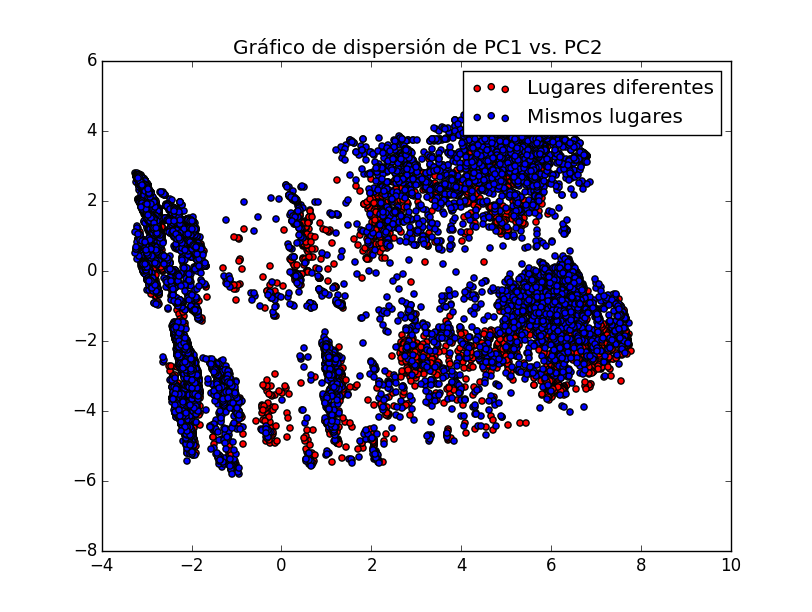
\includegraphics[width=10cm,keepaspectratio]{pca1_vs_pca2.png}
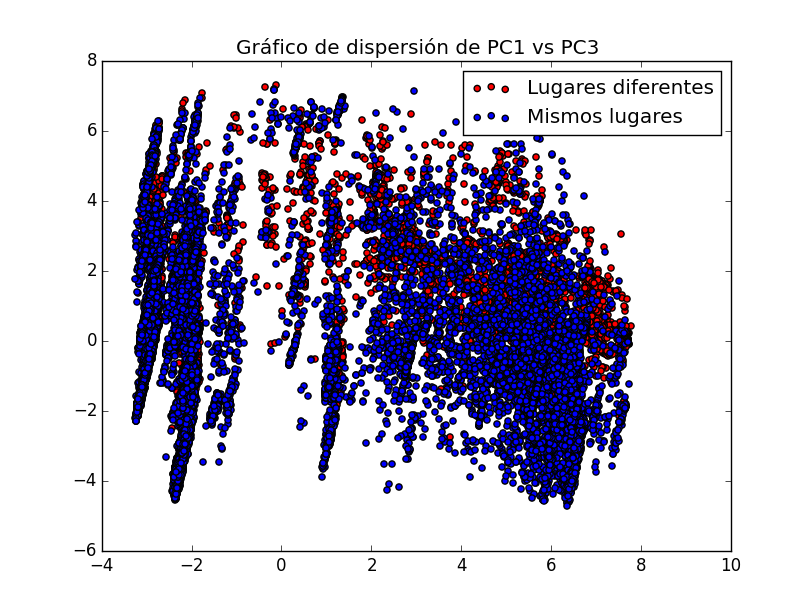
\includegraphics[width=10cm,keepaspectratio]{pca1_vs_pca3.png}
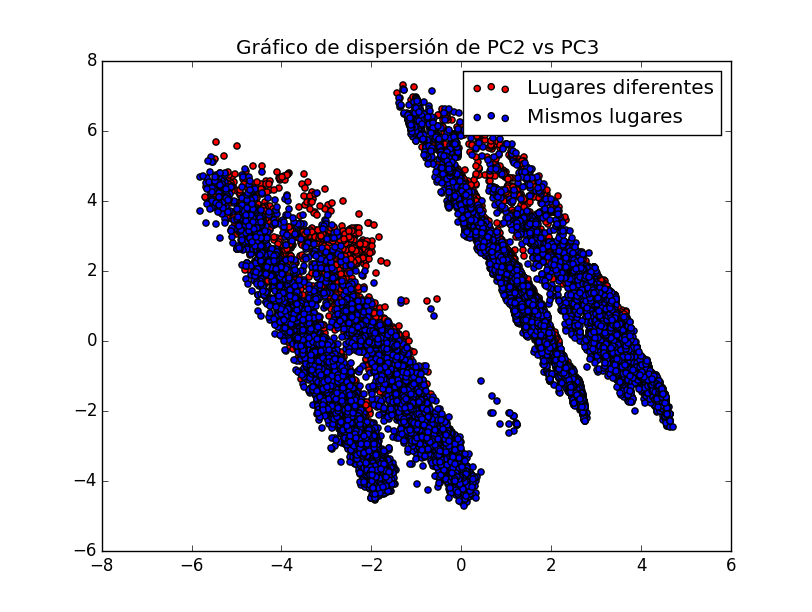
\includegraphics[width=10cm,keepaspectratio]{pca2_vs_pca3.png}
\end{figure}


La tabla \ref{table:main_results} muestra la efectividad en la clasificación
y los tiempos de ejecución de cada uno de los algoritmos descriptos en
la sección de \textit{Materiales}

El ensamble de 3 clasificadores tiene una performance del 97.78\%, y el
de 5 clasificadores del 98.07\%.

\begin{table}[!hb]
\caption{Performance con validación cruzada de todos los clasificadores}
\label{table:main_results}
\centering
\begin{tabular}{l | l l l | l l}
	Id	&	Clasificador	&	Grado	&    $\gamma$	& Tiempo [s]  &	Performance c/ \\
	&			&		&		&	Val. Cruzada	& Val. Cruzada\\
\hline
	1	&	LDA	&		&		&	12	&	\textbf{94.14} \\
\hline
	2	&	SVM lineal 	&		&		&	156	&	94.82 \\
	3 	&	SVM polinómico 	&	2	&	1	&	774	&	96.06 \\
	4 	&	SVM polinómico 	&	2	&	0	&	181	&	94.44 \\
	5 	&	SVM polinómico 	&	2	&	 $ 10^{-1} $  	&	138	&	96.13 \\
	6 	&	SVM polinómico 	&	2	&	 $ 10^{-2} $  	&	168	&	95.11 \\
	7 	&	SVM polinómico 	&	2	&	$ 10^{-4} $	&	404	&	92.44 \\
	8 	&	SVM polinómico 	&	2	&	 $ 10^{-4} $  	&	551	&	71.44 \\
	9 	&	SVM polinómico 	&	2	&	 $ 10^{-5} $  	&	487	&	71.44 \\
	10	&	SVM polinómico 	&	3	&	1	&	1369	&	94.57 \\
	11	&	SVM polinómico 	&	3	&	0	&	199	&	94.5 \\
	12	&	SVM polinómico 	&	3	&	 $ 10^{-1} $  	&	196	&	\textbf{96.14} \\
	13	&	SVM polinómico 	&	3	&	 $ 10^{-2} $  	&	157	&	95.35 \\
	14	&	SVM polinómico 	&	3	&	$ 10^{-4} $	&	524	&	71.44 \\
	15	&	SVM polinómico 	&	3	&	 $ 10^{-4} $  	&	474	&	71.44 \\
	16	&	SVM polinómico 	&	3	&	 $ 10^{-5} $  	&	477	&	71.44 \\
	17	&	SVM polinómico 	&	4	&	1	&	2005	&	93.65 \\
	18	&	SVM polinómico 	&	4	&	0	&	223	&	94.3 \\
	19	&	SVM polinómico 	&	4	&	 $ 10^{-1} $  	&	333	&	95.49 \\
	20	&	SVM polinómico 	&	4	&	 $ 10^{-2} $  	&	158	&	95.48 \\
	21	&	SVM polinómico 	&	4	&	$ 10^{-4} $	&	549	&	71.44 \\
	22	&	SVM polinómico 	&	4	&	 $ 10^{-4} $  	&	476	&	71.44 \\
	23	&	SVM polinómico 	&	4	&	 $ 10^{-5} $  	&	475	&	71.44 \\
	24	&	SVM polinómico 	&	5	&	1	&	2251	&	93.42 \\
	25	&	SVM polinómico 	&	5	&	0	&	252	&	94.05 \\
	26	&	SVM polinómico 	&	5	&	 $ 10^{-1} $  	&	450	&	94.99 \\
	27	&	SVM polinómico 	&	5	&	 $ 10^{-2} $  	&	150	&	95.56 \\
	28	&	SVM polinómico 	&	5	&	$ 10^{-4} $	&	530	&	71.44 \\
	29	&	SVM polinómico 	&	5	&	 $ 10^{-4} $  	&	476	&	71.44 \\
	30	&	SVM polinómico 	&	5	&	 $ 10^{-5} $  	&	473	&	71.44 \\
	31	&	SVM sigmoide 	&		&	1	&	666	&	60.89 \\
	32	&	SVM sigmoide 	&		&	0	&	451	&	71.44 \\
	33	&	SVM sigmoide 	&		&	 $ 10^{-1} $ 	&	787	&	60.76 \\
	34	&	SVM sigmoide 	&		&	 $ 10^{-2} $ 	&	446	&	72.39 \\
	35	&	SVM sigmoide 	&		&	$ 10^{-3} $	&	270	&	92.92 \\
	36	&	SVM sigmoide 	&		&	 $ 10^{-4} $ 	&	436	&	90.94 \\
	37	&	SVM sigmoide 	&		&	 $ 10^{-5} $ 	&	550	&	71.44 \\
\hline
	38	&	K-nn	&	3	&		&	68	&	\textbf{94.99} \\
	39	&	K-nn	&	4	&		&	68	&	94.61 \\
	40	&	K-nn	&	5	&		&	71	&	94.81 \\
	41	&	K-nn	&	6	&		&	70	&	94.58 \\
	42	&	K-nn	&	7	&		&	73	&	94.63 \\
	43	&	K-nn	&	8	&		&	74	&	94.5 \\
	44	&	K-nn	&	9	&		&	72	&	94.66 \\
	45	&	K-nn	&	10	&		&	74	&	94.53 \\
	46	&	K-nn	&	11	&		&	75	&	94.48 \\
	47	&	K-nn	&	12	&		&	76	&	94.28 \\
	48	&	K-nn	&	13	&		&	73	&	94.22 \\
	49	&	K-nn	&	14	&		&	76	&	94.1 \\
	50	&	K-nn	&	15	&		&	78	&	94.04 \\
	51	&	K-nn	&	16	&		&	74	&	93.9 \\
	52	&	K-nn	&	17	&		&	74	&	93.97 \\
	53	&	K-nn	&	18	&		&	78	&	93.83 \\
	54	&	K-nn	&	19	&		&	79	&	93.86 \\
	55	&	K-nn	&	20	&		&	75	&	93.78 \\
\hline
	56	& Regresión Log. &		&		&	11      &  \textbf{94.73} \\
\hline
	57	& Random forest	&		&		&	16	&  \textbf{96.89} \\
\hline
	58	&  ensemble de &	  	&		&		&	97.78 \\
		&  3 clasificadores &		&		&		&	      \\
\hline
	59	&  ensemble de &	  	&		&		&	98.07 \\
		&  5 clasificadores &		&		&		&	      \\

\end{tabular}
\end{table}


\section{Discusión}
\subsection{Análisis de Componentes Principales}
La tabla \ref{table:pca_results} muestra la varianza acumulada de las
primeras 30 componentes principales. La tabla muestra que el 95\%
de la varianza puede ser explicada con 17 componentes de las 118 variables
totales del dataset. Con 30 componentes principales, se puede explicar
el 99\% de la varianza.

Los gráficos de la figura \ref{fig:pca_scatterplot} muestran 3 
gráficos de dispersión de
las 3 primeras componentes principales. Los gráficos de la componente principal 1 
contra la componente 2 y 3, muestran que no se pueden identificar las clases, ya
que ambas estan distribuidas por todo el gráfico. En el gráfico de la
componente principal 2 y la 3 ya se puede ver que las clases que apuntan
a \textit{``lugares diferentes''}, se encuentran más agrupadas que en las componentes
previas. Sin embargo, pese al mayor poder de agrupamiento, estan muy juntas a
las instancias de la clase contraria, haciendo imposible una clara identificación por
componentes principales.

\subsection{Métodos de clasificación}
El objetivo que se persigue en este trabajo es encontrar varios clasificadores
de diferentes tipos, que tengan un buen desempeño encontrando las clases:
instancias que apuntan al mismo lugar y las que no. El objetivo final es apalancar
el desempeño de estos clasificadores individuales haciendo un ensamble
de los mejores de estos. 
Para esto se prueba clasificadores de diversas especies con distintos parámetros.
Se prueba con discriminantes lineal de Fisher, 
máquinas de vector soporte, K vecinos mas cercanos, regresión logística
y random forest. Se intenta en primera 
instancia encontrar el mejor clasificador de cada tipo. Luego, se verifica si
haciendo un ensamble de los mejores, la performance general es aún mejor.

Se aclara que todas las mediciones de performance en esta
sección son aplicando validación cruzada, a excepción de los ensembles.

\subsection{Análisis discriminante lineal de Fisher}
El clasificador por discriminante lineal de Fisher no requieren una combinación 
de parámetros para escoger el mejor. Este clasificador pudo diferenciar correctamente
el 94.14\% de las instancias. Como es el único clasificador de esta especie
y su capacidad predictiva es superior al 90\%, se lo selecciona para
formar parte de los ensembles.

\subsection{Máquinas de vector soporte}
Las máquinas de vector soporte son buenas clasificadoras para algunos problemas complejos, permiten
clasificar datos no lineales y en algunos casos tienen una perforance superior a la media.
Como contrapartida, son costosas de entrenar: consumen mucha  memoria y
demandan muchas operaciones de CPU (respecto a otros clasificadores), y además hay que encontrar
los parámetros empíricos que mejor se ajustan a los datos.  
Se intenta escoger el mejor modelo de maquinas de vector soporte. Se
decide probar con 3 kernels distintos y combinar parámetros sobre
cada uno de ellos, para escoger finalmente un modelo para formar parte
del ensamble definitivo. Se prueban los kerners: lineal, polinómico y
sigmoide. El modelo lineal, el más sencillo de todos y usado como referencia,
puede clasificar correctamente el 94.82\% de los datos. 
Se prueban los kernels polinómicos de $2^{\circ}$, $3^{\circ}$, $4^{\circ}$ y $5^{\circ}$ orden. A cada
uno de ellos se los corre con varios valores de $\gamma$ (entre 1 y $10^{-5}$) . Los modelos
con buen desempeño tienen una performance que oscilan entre el 92 y
96\%. Para todos los grados el mejor $\gamma$ es de $10^{-1}$, excepto para el polinómico
de $5^{\circ}$ orden, cuyo mejor $\gamma$ es de $10^{-2}$. 

Si se considera el mejor $\gamma$ de cada kernel polinómico, todos los modelos tienen un
desempeño de entre el 95\% y 96\%.

Respecto a los tiempos de ejecución, estos crecen sensiblemente a medida que el $\gamma$ 
disminuye. Esto se debe a que mientras menor sea el $\gamma$, mayor es la precisión que 
se le exige al modelo y hay que realizar  mas cálculos aritméticos para encontrar
el polinomio discriminante. 

Respecto al kernel sigmoide, solo se obtiene buenos resultados con $\gamma=10^{-3}$
y $\gamma=10^{-4}$. Para los demás $\gamma$, la performance es del orden del
70\%.

Tras evaluar los 36 modelos distintos de máquinas de vector soporte, se escoge
el del kernel polinómico de grado 3 y $\gamma=10^{-1}$ porque tiene una performance del
96.14\%, siendo este el mejor de todos.

\subsection{K vecinos mas cercanos}
Se realizan corridas de K vecinos más cercanos, iterando con K desde
3 a 20 y distancia de Minkowski. En todos los casos se clasificaron
correctamente entre el 93\% y 95\% de las instancias. Los tiempos de corrida aumentaron
a medida que K aumentaba, pero siempre estos tiempos son sensiblemente
mas bajos que los de máquinas de vector soporte.

Lo curioso de este clasificador es que para este problema puntual, a medida
que aumenta el K, disminuye la capacidad de predicción. Posiblemente
lo que sucede es que como el dataset contiene muchas variables, 
los datos estan en un espacio de muchas dimensiones, 
tendiendo a estar alejados entre si, de manera que
el vecindario esta formado por puntos lejanos.
De cualquier modo, la mayor diferencia por variación del K 
 no es mayor al 1.20\%.

Se escoge el clasificador con K=3 para ser usado en el ensemble final,
porque su performance del 94.99\% es la mayor de esta especie.

\subsection{Regresión logística}
La regresión logística que no descarta ninguna variable tiene 
una capacidad predictiva del 94.73\%, equivalente a la del
discriminante lineal de Fisher.

\subsection{Random forest}
Random forest de por si ya es un ensemble de varios arboles
CART. La performance de este algortimo es del 96.89\%,
siendo el algoritmo de mayor poder de discriminación  individual. 

Hay que destacar que random forest no solo supero en capacidad preditiva
al mejor SVM, sino que en tiempo de corrida fue ampliamente superior:
Random Forest fue entrenado en 16 segundos, mientras que SVN requirió
196. De todas formas, se debe tener en cuenta que el nivel de
concurrencia de random forest es superior al de SVM.

\subsection{Ensembles}
La tabla \ref{table:ensemble_summary} resume la performance
de los 5 clasificadores bases y los ensambles. 
Estos últimos son construido por votos, lo que
significa que la clase seleccionada es la escogida por la mayoría 
de los clasificadores.

\begin{table}[ht!]
\caption{Clasificadores individuales y ensembles}
\label{table:ensemble_summary}
\centering
\begin{tabular}{l | l l l }
Tipo & Performance  \\
\hline
LDA & 94.14 \\
SVM polinómico & 96.14 \\
K-nn & 94.99 \\
Reg. log. & 94.73 \\
Random forest & 96.89 \\
\hline
Ensemble de 3 clasif. & 97.78 \\
Ensemble de 5 clasif. & 98.07 \\
\end{tabular}
\end{table}

Lo mas importante es que la eficiencia del peor de los ensemble
es superior al mejor de los clasificadores individuales, inclusive
que a random forest, que es un ensemble de arboles CART.

La performance del ensamble de 3 clasificadores es de un 97.78\%, 
superior a todos los clasificadores individuales. Usando
5 clasificadores en vez de 3, e incluyendo a random forest, el clasificador de 
mejor potencia predictiva, la ganancia en clasificación es marginal: 0.29\%.

Se recuerda que los ensembles son las únicas
mediciones que no se realiza validación cruzada, sino que el 
procedimiento es separando una muestra de un 20\% para testeo y
entrenando nuevamente  los clasificadores del ensamble con el 80\%
de entrenamiento.

Se ha intentado mejorar la performance usando mas clasificadores de
máquinas vector soporte o K vecinos mas cercanos, obteniendo los
mismos resultados. 

\section{Conclusiones}
Se ha logrado construir un ensemble de clasificadores capaz de identificar
con un 98.07\% de precisión si los atributos de lugares de dos registros
referencian al mismo lugar o no,
usando los datos transformados y provistos por el motor de búsqueda de Nomao.

\section*{Agradecimientos}
Se agradece a Marcelo Soria por el tiempo, dedicación y esfuerzo 
revisando, aconsejando y corrigiendo este trabajo, 
con el que me recibo de Especialista
en Data Mining.


\appendices

\section{Especificación de los datos provistos por Nomao}
\label{appendix1}
La tabla \ref{table:data_set} lista todas las variables provistas por la
organización como su tipo. Todas las variables 
categóricas pueden tener 3 valores posibles:
\textit{'n'}, \textit{'s'} o \textit{'m'}.
Todas las variables continuas son reales con valores entre 
0 y 1. Las variables continuas pueden tener valores faltantes.

\begin{table}[ht!]
\caption{Descripcion de las 118 variables} 
\label{table:data_set}
\begin{tabular}{l | l l }
Numero & Nombre & Tipo \\
       &        &      \\
\hline
1	& id  & string  \\
2	& clean\_name\_intersect\_min  &   real  \\
3	& clean\_name\_intersect\_max  &   real  \\
4	& clean\_name\_levenshtein\_sim  &   real  \\
5	& clean\_name\_trigram\_sim  &   real  \\
6	& clean\_name\_levenshtein\_term  &   real  \\
7	& clean\_name\_trigram\_term  &   real  \\
8	& clean\_name\_including  &    categorica   \\
9	& clean\_name\_equality  &    categorica   \\
10	& city\_intersect\_min  &   real  \\
11	& city\_intersect\_max  &   real \\
12	& city\_levenshtein\_sim  &   real  \\
13	& city\_trigram\_sim  &   real  \\
14	& city\_levenshtein\_term  &   real  \\
15	& city\_trigram\_term  &   real  \\
16	& city\_including  &    categorica   \\
17	& city\_equality  &    categorica   \\
18	& zip\_intersect\_min  &   real  \\
19	& zip\_intersect\_max  &   real  \\
20	& zip\_levenshtein\_sim  &   real  \\
21	& zip\_trigram\_sim  &   real  \\
22	& zip\_levenshtein\_term  &   real  \\
23	& zip\_trigram\_term  &   real  \\
24	& zip\_including  &    categorica   \\
25	& zip\_equality  &    categorica   \\
26	& street\_intersect\_min  &   real  \\
27	& street\_intersect\_max  &   real  \\
28	& street\_levenshtein\_sim  &   real  \\
29	& street\_trigram\_sim  &   real  \\
30	& street\_levenshtein\_term  &   real  \\
31	& street\_trigram\_term  &   real  \\
32	& street\_including  &    categorica   \\
33	& street\_equality  &    categorica   \\
34	& website\_intersect\_min  &   real  \\
35	& website\_intersect\_max  &   real  \\
36	& website\_levenshtein\_sim  &   real  \\
37	& website\_trigram\_sim  &   real  \\
38	& website\_levenshtein\_term  &   real  \\
39	& website\_trigram\_term  &   real  \\
40	& website\_including  &    categorica   \\
41	& website\_equality  &    categorica   \\
42	& countryname\_intersect\_min  &   real  \\
43	& countryname\_intersect\_max  &   real  \\
44	& countryname\_levenshtein\_sim  &   real  \\
45	& countryname\_trigram\_sim  &   real  \\
46	& countryname\_levenshtein\_term  &   real  \\
47	& countryname\_trigram\_term  &   real  \\
48	& countryname\_including  &    categorica   \\
49	& countryname\_equality  &    categorica   \\
50	& geocoderlocalityname\_intersect\_min  &   real  \\
51	& geocoderlocalityname\_intersect\_max  &   real  \\
52	& geocoderlocalityname\_levenshtein\_sim  &   real  \\
53	& geocoderlocalityname\_trigram\_sim  &   real  \\
54	& geocoderlocalityname\_levenshtein\_term  &   real  \\
55	& geocoderlocalityname\_trigram\_term  &   real  \\
56	& geocoderlocalityname\_including  &    categorica   \\
57	& geocoderlocalityname\_equality  &    categorica   \\
58	& geocoderinputaddress\_intersect\_min  &   real  \\
59	& geocoderinputaddress\_intersect\_max  &   real  \\
60	& geocoderinputaddress\_levenshtein\_sim  &   real  \\
61	& geocoderinputaddress\_trigram\_sim  &   real  \\
62	& geocoderinputaddress\_levenshtein\_term  &   real  \\
63	& geocoderinputaddress\_trigram\_term  &   real  \\
64	& geocoderinputaddress\_including  &    categorica   \\
65	& geocoderinputaddress\_equality  &    categorica   \\
66	& geocoderoutputaddress\_intersect\_min  &   real  \\
67	& geocoderoutputaddress\_intersect\_max  &   real  \\
68	& geocoderoutputaddress\_levenshtein\_sim  &   real  \\
69	& geocoderoutputaddress\_trigram\_sim  &   real  \\
70	& geocoderoutputaddress\_levenshtein\_term  &   real  \\
\end{tabular}
\end{table}

\begin{table}[ht!]
\centering
\begin{tabular}{l | l l l}
Numero & Nombre & Tipo & Rango \\
       &        &      &                 \\
\hline
71	& geocoderoutputaddress\_trigram\_term  &   real  \\
72	& geocoderoutputaddress\_including  &    categorica   \\
73	& geocoderoutputaddress\_equality  &    categorica   \\
74	& geocoderpostalcodenumber\_intersect\_min  &   real  \\
75	& geocoderpostalcodenumber\_intersect\_max  &   real  \\
76	& geocoderpostalcodenumber\_levenshtein\_sim  &   real  \\
77	& geocoderpostalcodenumber\_trigram\_sim  &   real  \\
78	& geocoderpostalcodenumber\_levenshtein\_term  &   real  \\
79	& geocoderpostalcodenumber\_trigram\_term  &   real  \\
80	& geocoderpostalcodenumber\_including  &    categorica   \\
81	& geocoderpostalcodenumber\_equality  &    categorica   \\
82	& geocodercountrynamecode\_intersect\_min  &   real  \\
83	& geocodercountrynamecode\_intersect\_max  &   real  \\
84	& geocodercountrynamecode\_levenshtein\_sim  &   real  \\
85	& geocodercountrynamecode\_trigram\_sim  &   real  \\
86	& geocodercountrynamecode\_levenshtein\_term  &   real  \\
87	& geocodercountrynamecode\_trigram\_term  &   real  \\
88	& geocodercountrynamecode\_including  &    categorica   \\
89	& geocodercountrynamecode\_equality  &    categorica   \\
90	& phone\_diff  &   real  \\
91	& phone\_levenshtein  &   real  \\
92	& phone\_trigram  &   real  \\
93	& phone\_equality  &    categorica   \\
94	& fax\_diff  &   real  \\
95	& fax\_levenshtein  &   real  \\
96	& fax\_trigram  &   real  \\
97	& fax\_equality  &    categorica   \\
98	& street\_number\_diff  &   real  \\
99	& street\_number\_levenshtein  &   real  \\
100	& street\_number\_trigram  &   real  \\
101	& street\_number\_equality  &    categorica   \\
102	& geocode\_coordinates\_long\_diff  &   real  \\
103	& geocode\_coordinates\_long\_levenshtein  &   real  \\
104	& geocode\_coordinates\_long\_trigram  &   real  \\
105	& geocode\_coordinates\_long\_equality  &    categorica   \\
106	& geocode\_coordinates\_lat\_diff  &   real  \\
107	& geocode\_coordinates\_lat\_levenshtein  &   real  \\
108	& geocode\_coordinates\_lat\_trigram  &   real  \\
109	& geocode\_coordinates\_lat\_equality  &    categorica   \\
110	& coordinates\_long\_diff  &   real  \\
111	& coordinates\_long\_levenshtein  &   real  \\
112	& coordinates\_long\_trigram  &   real  \\
113	& coordinates\_long\_equality  &    categorica   \\
114	& coordinates\_lat\_diff  &   real  \\
115	& coordinates\_lat\_levenshtein  &   real  \\
116	& coordinates\_lat\_trigram  &   real  \\
117	& coordinates\_lat\_equality  &    categorica   \\
118	& geocode\_coordinates\_diff  &   real  \\
119	& coordinates\_diff  &   real  \\
120	& label (clase) & categorica (1 o 0). \\
\end{tabular}
\end{table}

\section{Referencias}
\label{appendix2}
[1] Jolliffe, I. T. (1986). Principal Component Analysis. Springer-Verlag.

[2]Mosteller F. and Tukey J.W. Data analysis, including statistics. In Handbook of Social Psychology. Addison-Wesley, Reading, MA, 1968.

[3]Geisser, Seymour (1993). Predictive Inference. New York, NY: Chapman and Hall. ISBN 0-412-03471-9.

[4]Kohavi, Ron (1995). ``A study of cross-validation and bootstrap for accuracy estimation and model selection''. Proceedings of the Fourteenth International Joint Conference on Artificial Intelligence (San Mateo, CA: Morgan Kaufmann) 2 (12): 1137–1143. CiteSeerX: 10.1.1.48.529.

[5] Devijver, Pierre A.; Kittler, Josef (1982). Pattern Recognition: A Statistical Approach. London, GB: Prentice-Hall.

[6] Fisher, R. A. (1936). ``The Use of Multiple Measurements in Taxonomic Problems''. Annals of Eugenics 7 (2): 179–188. doi:10.1111/j.1469-1809.1936.tb02137.x. hdl:2440/15227.

[7] McLachlan, G. J. (2004). Discriminant Analysis and Statistical Pattern Recognition. Wiley Interscience. ISBN 0-471-69115-1. MR 1190469.

[8] Cortes, C.; Vapnik, V. (1995). ``Support-vector networks''. Machine Learning 20 (3): 273. doi:10.1007/BF00994018.

[9] Altman, N. S. (1992). ``An introduction to kernel and nearest-neighbor nonparametric regression''. The American Statistician 46 (3): 175–185. doi:10.1080/00031305.1992.10475879

[10]  Walker, SH; Duncan, DB (1967). ``Estimation of the probability of an event as a function of several independent variables''. Biometrika 54: 167–178.

[11] Cox, DR (1958). ``The regression analysis of binary sequences (with discussion)''. J Roy Stat Soc B 20: 215–242.

[12] Breiman, Leo (2001). ``Random Forests''. Machine Learning 45 (1): 5–32. doi:10.1023/A:1010933404324.


\end{document}

